\documentclass[catalan]{scrartcl}

% encoding
\usepackage[utf8]{inputenc}
\usepackage[T1]{fontenc}
\usepackage{lmodern}
\usepackage{babel}

% formatting and fixes
\frenchspacing
\usepackage[style=spanish]{csquotes}
\MakeAutoQuote{«}{»}

% general design preferences (page, paragraph indent/space, margins, class options, ...)
\setlength{\parskip}{10pt}
\setlength{\parindent}{0pt}
%\pagestyle{plain}

% ADD ANY SPECIFIC PACKAGES HERE
% (CHEMISTRY, CODE, PUBLISHING)
\usepackage{siunitx}
\usepackage{tikz}
\usepackage{mathtools}
\usepackage{nicefrac}
\usepackage{minted}

% other options

%\usemintedstyle{xcode}
\setminted{
  %frame=leftline,
  %framesep=12pt,
  xleftmargin=15pt,
}

% hyperlink setup / metadata
\usepackage{hyperref}
\AfterPreamble{\hypersetup{
  pdftitle={Memòria P1 — PSAVC QP2019},
  %pdfsubject={PSAVC},
}}

% document metadata
\author{Alba Mendez}
\title{Memòria pràctica 1\\
{\small PSAVC QP2019}}
\date{24 de març de 2019}

\begin{document}

%\begin{minipage}{\columnwidth}
\maketitle
%\end{minipage}


\part{Introducció}

En aquesta pràctica es planteja un escenari on tenim un \emph{emissor}
que emet fotons amb una velocitat mitjana $\lambda$, que varia segons
si s'està transmetent un bit~0 ($\lambda = \lambda_0$) o un bit~1
($\lambda = \lambda_1$).

La distribució d'emissió dels fotons segueix un procés de Poisson, i per
tant la quantitat $N(t)$ de fotons emesos en un temps $t$ segueix una
distribució de Poisson, amb la funció de probabilitat:
%
\begin{equation}
  P[N(t) = n] = e^{-\lambda t} \frac{\left(\lambda t\right)^n}{n!}
\end{equation}

Però nosaltres no podem mesurar directament $N(t)$, sino que fem servir
un \emph{detector} òptic que mesura cada fotó amb una probabilitat
independent $p$. El detector ens retorna el nombre de fotons $M(t)$
mesurats en el temps $t$.

Com es demostrarà en l'estudi previ, l'estadística de $M(t)$ és també
una distribució de Poisson igual que $N(t)$, només que amb
$\lambda' = \lambda p$. La seva funció de probabilitat és:
%
\begin{equation}
  P[M(t) = m] = e^{-\lambda p t} \frac{\left(\lambda p t\right)^m}{m!}
\end{equation}

L'objectiu de la pràctica és elaborar un detector per determinar, a partir
de $M$ i fixats $t$, $\lambda_0$, $\lambda_1$ i $p$, si s'està transmetent
un 0 o un 1 i estudiar les seves característiques. El detector es dissenyarà
partint del criteri Neyman-Pearson; s'estudiarà la seva ROC teòrica i es
duran a terme simulacions de Montecarlo per a calcular de forma empírica la
probabilitat de detecció i de falsa alarma per un cas concret. Els bits són
equiprobables.


\part{Estudi previ}

\paragraph{Qüestió 1.1.}

Es demana demostrar que $M(t)$ es una v.a. de Poisson amb paràmetre $\lambda p$.

Per fer-ho, suposem que $N(t)$ no és aleatori. Llavors, $M(t)$ segueix
una distribució binomial, és la quantitat d'encerts entre $N(t)$ processos de Bernoulli amb probabilitat $p$. Per tant, podem escriure la funció de
probabilitat de $M(t)$ condicionada a $N(t)$ com:
%
\begin{align}
  P\left[ M(t) = m \Bigr\rvert_{N(t) = n} \right] &=
    \frac{n!}{m! \, (n - m)!} \, p^m \, (1-p)^{n-m}
\end{align}
%
D'aquí podem extreure la funció de probabilitat conjunta:
%
\begin{align}
  P[ M(t) = m \cap N(t) = n ] &=
    P[N(t) = n] \cdot P\left[ M(t) = m \Bigr\rvert_{N(t) = n} \right]
\\
  &=
    e^{-\lambda t} \frac{\left(\lambda t\right)^n}{n!}
    \cdot
    \frac{n!}{m! \, (n - m)!} \, p^m \, (1-p)^{n-m}
\\
  &=
    e^{-\lambda t} \frac{\left(\lambda t\right)^n}{m! \, (n - m)!}
    \, p^m \, (1-p)^{n-m}
\end{align}
%
De la funció de probabilitat conjunta, integrem sobre tots els valors de
$N(t)$ per obtenir la funció de probabilitat de $M(t)$:
%
\begin{align}
  P[ M(t) = m ] &=
    \sum_{n = -\infty}^{n = \infty} P[ M(t) = m \cap N(t) = n ]
\\
  &=
    e^{-\lambda t} \, \frac{p^m}{m!} \, \sum_{n = -\infty}^{n = \infty}
    \frac{\left(\lambda t\right)^n}{(n - m)!} (1-p)^{n-m}
\end{align}
%
Fem un canvi de variable $k = n - m$ al sumatori:
%
\begin{align}
  \hphantom{ P[ M(t) = m ] } &=
    e^{-\lambda t} \, \frac{p^m}{m!} \, \sum_{k = -\infty}^{k = \infty}
    \frac{\left(\lambda t\right)^{k+m} }{k!} (1-p)^k
\\
  &=
    e^{-\lambda t} \, \frac{p^m \left(\lambda t\right)^m}{m!}
    \, \sum_{k = -\infty}^{k = \infty}
    \frac{\left(\lambda t\right)^{k} (1-p)^k }{k!}
\\
  &=
    e^{-\lambda t} \, \frac{\left(\lambda p t\right)^m}{m!}
    \, \sum_{k = -\infty}^{k = \infty}
    \frac{\left[\lambda t (1-p)\right]^{k} }{k!}
\end{align}
%
D'aquí, com que $k!$ no està definit per a enters negatius, podem modificar el límit inferior del sumatori a $k = 0$. Identifiquem que el sumatori és la sèrie de Taylor de $e^{\lambda t (1-p)}$:
%
\begin{align}
  \hphantom{ P[ M(t) = m ] } &=
    e^{-\lambda t} \, \frac{\left(\lambda p t\right)^m}{m!}
    \, e^{\lambda t (1-p)}
\\
  &=
    e^{-\lambda p t} \, \frac{\left(\lambda p t\right)^m}{m!}
\end{align}

Queda demostrat.

\paragraph{Qüestió 1.2.}

Ara es demana trobar el detector de Neyman-Pearson:
%
\begin{align}
  \frac{P\left[ M(T) = m \Bigr\rvert_{H_1} \right]}
       {P\left[ M(T) = m \Bigr\rvert_{H_0} \right]} > \gamma
\end{align}
%
tal que $P_{FA} \leq \alpha$, i donar les expressions de $P_{FA}$ i $P_{D}$.

Per començar, calcularem la funció estadística del detector. \textbf{Assumirem que $\lambda_1 > \lambda_0$}, cosa que no ens fa perdre generalitat:
%
\begin{align}
  \frac{e^{-\lambda_1 p T} \, \frac{\left(\lambda_1 p T\right)^m}{m!}}
       {e^{-\lambda_0 p T} \, \frac{\left(\lambda_0 p T\right)^m}{m!}}
       &> \gamma
\\
  e^{-(\lambda_1-\lambda_0) p T} \,
  \frac{ \left(\lambda_1 p T\right)^m }{ \left(\lambda_0 p T\right)^m }
  &> \gamma
\\
  \left( \nicefrac{ \lambda_1 }{ \lambda_0 } \right)^m
  &> e^{(\lambda_1-\lambda_0) p T} \, \gamma
\\
  m &> \frac{ (\lambda_1-\lambda_0) p T + \ln \gamma }{ \ln \nicefrac{ \lambda_1 }{ \lambda_0 } } = \gamma'
\end{align}
%
Ara calculem $P_{FA}$ en funció del llindar $\gamma'$:
%
\begin{align*}
  P_{FA} &= P\left[ M(T) > \gamma' \Bigr\rvert_{H_0} \right]
  = 1 - P\left[ M(T) \leq \gamma' \Bigr\rvert_{H_0} \right]
  = 1 - F(\gamma'; \lambda_0 p T)
\end{align*}
%
On $F(n;\lambda)$ és la funció cumulativa d'una v.a. de Poisson amb paràmetre $\lambda$. \\
Seguim el mateix procediment per a $P_D$. Les probabilitats són per tant:
%
\begin{align*}
  P_{FA} = 1 - F(\gamma'; \lambda_0 p T) \quad\quad P_D &= 1 - F(\gamma'; \lambda_1 p T)
\end{align*}
%
Ara només cal triar el llindar apropiat segons $\alpha$, que seria $
%1 - F(\gamma'; \lambda_0 p T) \leq \alpha \Leftrightarrow
\gamma' = F^{-1}(1 - \alpha; \lambda_0 p T)$, on definim que
$F^{-1}(x)$ retorna l'enter més petit $k$ que compleix $F(k) \geq x$.


\part{Activitat al laboratori}

Durant tota l’activitat es treballarà amb $\lambda_0 = 2$, $\lambda_1 = 5$
i $p = 0.8$.

\paragraph{Activitat 1.1.}

En aquesta primera activitat es demana que amb $T = 5$ obtinguem el valor
del llindar $\gamma'$ del detector, per tal que $P_{FA} \leq 0.05$.

\begin{minted}{matlab}
T = 5;
alpha = 0.05;
\end{minted}

En primer lloc farem servir \mintinline{matlab}|poissinv| per calcular
$\gamma'$:

\begin{minted}{matlab}
gamma_p = poissinv(1 - alpha, lambda0 * p * T)
\end{minted}

En resulta que $\gamma' = 13$. Ara calcularem $P_{FA}$ i $P_D$ mitjançant
la funció \mintinline{matlab}|poisscdf|:

\begin{minted}{matlab}
P_FA = 1 - poisscdf(gamma_p, lambda0 * p * T)
P_D  = 1 - poisscdf(gamma_p, lambda1 * p * T)
\end{minted}

Obtenim $P_{FA} = 0.0342; P_D = 0.9339$. Com que la variable sobre la que
treballa el detector ($M(t)$) té valors discrets, el llindar també té valors
discrets i no existeix un detector amb $P_{FA}$ exactament igual a $0.05$.
En aquest cas, el que més s'apropa seguint el criteri de Neyman-Pearson té
$P_{FA} = 0.0342$.

\paragraph{Activitat 1.2.}

Ara es demana fer una simulació i extreure'n les probabilitats empíriques.
En primer pas, hem de generar una seqüència de $10^4$ bits equiprobables
($p_b = 0.5$):

\begin{minted}{matlab}
bit = rand(1, 1e4) >= 0.5;
\end{minted}

Ara cal simular el valor de $M(T)$ que s'acaba rebent al detector per a
cadascun dels bits. Això ho farem mitjançant la funció
\mintinline{matlab}|poissrnd| i associant cada bit al parámetre
de la distribució ($\lambda_0pT$ o $\lambda_1pT$) segons correspongui:

\begin{minted}{matlab}
lambdaK = [ lambda0, lambda1 ];
M = poissrnd(lambdaK(bit+1) * p * T);
\end{minted}

Llavors apliquem el llindar que hem obtingut abans per a obtenir el bit detectat:

\begin{minted}{matlab}
out_bit = M > gamma_p;
\end{minted}

Ara es demana calcular la $P_{FA}$ i la $P_D$ empíriques:

\begin{minted}{matlab}
P_FA_p = probability(out_bit(~bit))
P_D_p  = probability(out_bit(bit))
\end{minted}

On la funció \mintinline{matlab}|probability|, que donat un vector
lògic retorna la fracció de casos en que es compleix, es defineix de la forma següent:

\begin{minted}{matlab}
function p = probability(x)
    p = nnz(x) / numel(x);
end
\end{minted}

Les probabilitats obtingudes són $P_{FA}' = 0.0321; P_D' = 0.9403$.
S'assemblen força a les probabilitats teòriques, i de fet, si
fem diverses realitzacions podem veure que oscil·len al voltant d'aquests
valors. La variabilitat és esperada tenint en compte que el nombre de mostres.
Per tant, tot sembla correcte.

\paragraph{Activitat 1.3.}

Per a la última part es demana dibuixar la corba ROC per a diversos valors
de $T$. En primer lloc inicialitzarem uns eixos buits i activarem el
\emph{hold} per a pintar les successives línies:

\begin{minted}{matlab}
axes
xlabel('P_{FA}');
ylabel('P_D');
hold on
\end{minted}

Ara mitjançant un bucle iterarem sobre els diferents valors de $T$ i per a cadascun, calcularem les probabilitats per a diferents valors de $\gamma'$
i dibuixarem la corba resultant:

\begin{minted}{matlab}
for T = 1:0.5:10
    gamma_p = 0:70;
    P_FA = 1 - poisscdf(gamma_p, lambda0 * p * T);
    P_D  = 1 - poisscdf(gamma_p, lambda1 * p * T);
    plot(P_FA, P_D);
end
\end{minted}

\begin{figure}
\center
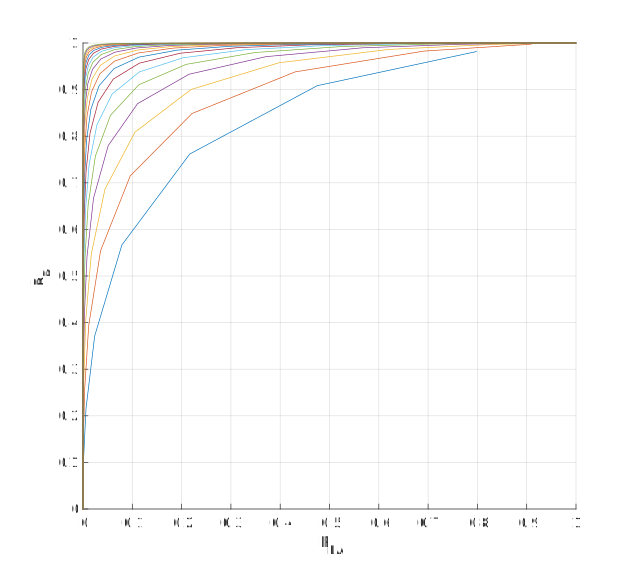
\includegraphics[width=\textwidth]{../roc.pdf}
\caption{ROC del detector per a diferents valors de $T$. \label{fig:roc}}
\end{figure}

El gràfic resultant es pot veure a la figura~\ref{fig:roc}. S'aprecia
com la corba amb la $T$ més baixa és la menys pronunciada (per tant, on
el detector és menys eficient) i les següents corbes tendeixen ràpidament
cap a la cantonada del gràfic. Aquestes corbes tan pronunciades es corresponen
amb les probabilitats obtingudes en les activitats anteriors.


\clearpage
\part*{Annex. Codi MATLAB}

%El codi emprat per a la realització de la pràctica es troba a continuació:

\begin{minted}{matlab}
lambda0 = 2;
lambda1 = 5;
p = 0.8;

%% Activitat 1

T = 5;
alpha = 0.05;

gamma_p = poissinv(1 - alpha, lambda0 * p * T)
P_FA = 1 - poisscdf(gamma_p, lambda0 * p * T)
P_D  = 1 - poisscdf(gamma_p, lambda1 * p * T)

%% Activitat 2

bit = rand(1, 1e4) >= 0.5;
lambdaK = [ lambda0, lambda1 ];
M = poissrnd(lambdaK(bit+1) * p * T);
out_bit = M > gamma_p;

P_FA_p = probability(out_bit(~bit))
P_D_p  = probability(out_bit(bit))

%% Activitat 3

axes
xlabel('P_{FA}');
ylabel('P_D');
grid on
hold on

for T = 1:0.5:10
    gamma_p = 0:70;
    P_FA = 1 - poisscdf(gamma_p, lambda0 * p * T);
    P_D  = 1 - poisscdf(gamma_p, lambda1 * p * T);
    plot(P_FA, P_D);
end

hold off

%% Utilitats

function p = probability(x)
    p = nnz(x) / numel(x);
end
\end{minted}


\end{document}
